% Created 2021-01-24 Sun 22:50
% Intended LaTeX compiler: pdflatex
\documentclass[11pt]{article}
\usepackage[utf8]{inputenc}
\usepackage[T1]{fontenc}
\usepackage{graphicx}
\usepackage{grffile}
\usepackage{longtable}
\usepackage{wrapfig}
\usepackage{rotating}
\usepackage[normalem]{ulem}
\usepackage{amsmath}
\usepackage{textcomp}
\usepackage{amssymb}
\usepackage{capt-of}
\usepackage{hyperref}
\usepackage{minted}
\hypersetup{colorlinks=true, linkcolor=black, filecolor=red, urlcolor=blue}
\usepackage[turkish]{babel}
\author{Eren Hatırnaz}
\date{29 Eylül 2019}
\title{Yazılım Gündemi - 11\\\medskip
\large 23-29 Eylül 2019}
\hypersetup{
 pdfauthor={Eren Hatırnaz},
 pdftitle={Yazılım Gündemi - 11},
 pdfkeywords={},
 pdfsubject={},
 pdfcreator={Emacs 27.1 (Org mode 9.3)},
 pdflang={Turkish}}
\begin{document}

\maketitle
\tableofcontents \clearpage\shorthandoff{=}

\begin{center}
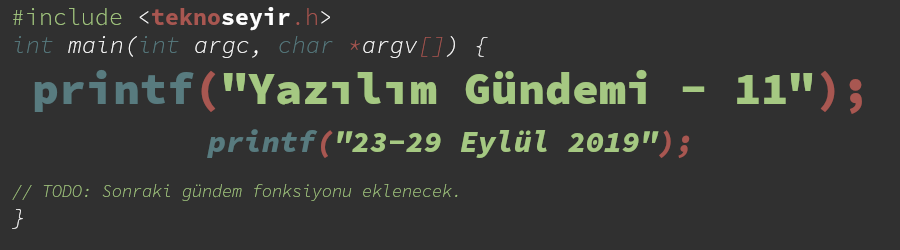
\includegraphics[width=.9\linewidth]{gorseller/yazilim-gundemi-banner.png}
\end{center}

\begin{center}
\href{../10/yazilim-gundemi-10.pdf}{< Önceki Gündem} | \textbf{23-29 Eylül 2019} | \href{../12/yazilim-gundemi-12.pdf}{Sonraki Gündem >}

\href{https://teknoseyir.com/blog/yazilim-gundemi-11-23-29-eylul-2019}{TeknoSeyir'de Oku}
\end{center}

\section{GitHub, \href{https://github.blog/2019-09-26-introducing-the-codesearchnet-challenge/}{CodeSearchNet projesini} duyurdu}
\label{sec:org3723ac5}
Veri, çağımızın en değerli şeyi haline gelirken GitHub'da elindeki kod
veritabanını değerlendirmeye çalışıyor. Bu çalışmalar doğrultusunda da semantik
şekilde kod araması yapabileceğimiz bir sistem üzerine geliştirmeler
yapıyorlarmış. CodeSearchNet ismini verdikleri bu projede henüz kullanılabilir
arayüzü olan bir arama motoru çıkmasa da, deneyimlerini aktarmak için
CodeSearchNet projesinde kullanılan verileri ve geliştirdikleri sistemi test
etmek için yarattıkları benchmark yönteminig tanıttılar. Böylece konuyla
ilgilenen diğer araştırmacılar da bu verileri ve yöntemleri kullanabilecekler.

Akademik makaleye ulaşmak için \href{https://arxiv.org/abs/1909.09436}{buraya} tıklayabilirsiniz.
\section{.NET Core \href{https://devblogs.microsoft.com/dotnet/announcing-net-core-3-0/}{3.0 duyuruldu}}
\label{sec:orge5ce025}
Microsoft'un son birkaç senedir üzerinde fazla yoğunlaştığı açık kaynaklı
uygulama çatısı .NET Core 3.0 sürümü bu hafta duyuruldu. Uzun zamandır .NET
tarafında geliştirme yapmıyorum fakat .NET Core uygulama çatısı, özellikle
GNU/Linux sistemlerde de çalışma özelliğine sahip olduğu için ilgimi çekiyor.
Bir ara inceleyeceğim. Ayrıca bu yeni sürüm birkaç aydır \href{https://dot.net}{dot.net} sitesinde ve
bing arama motorunda kullanılıyormuş, oralarda test etmişler yani.

Bu sürümle gelen bazı değişiklikler ise şu şekilde:
\begin{itemize}
\item C\# 8 ve F\# 4.7 desteği,
\item Hem Windows Forms olarak hem de WPF olarak Windows masaüstü uygulaması
geliştirebilme,
\item .NET Core uygulamaları artık varsayılan olarak çalıştırabilir (executable)
formatta olacak. Yani artık uygulama çalıştırmak için \texttt{dotnet myapp.dll}
yazmak yerine direkt \texttt{./myapp} yazarak çalıştırılabilecekler.
\item Yüksek performanslı JSON API sistemi eklenmiş.
\item Çöp toplayıcı (Garbage Collector) artık daha az bellek kullanıyor.
\end{itemize}

Visual Studio kullanıcıları bu sürümü kullanmak için Visual Studio 2019 16.3
sürümünü kullanmak zorundalar. Diğer özellikler için mutlaka konu başlığına
eklediğim bağlantıya tıklayınız.
\section{Yaklaşan Etkinlikler}
\label{sec:org62d6dc3}
\begin{longtable}{|p{8cm}|l|l|}
\hline
Etkinlik İsmi & Yer & Tarihi\\
\hline
\endfirsthead
\multicolumn{3}{l}{Önceki sayfadan devam ediyor} \\
\hline

Etkinlik İsmi & Yer & Tarihi \\

\hline
\endhead
\hline\multicolumn{3}{r}{Devamı sonraki sayfada} \\
\endfoot
\endlastfoot
\hline
\href{https://kommunity.com/software-craftsmanship-turkey/events/bash-lingua-non-grata}{BASH: Lingua Non Grata} & İstanbul & 2 Ekim 19:00\\
\href{https://kommunity.com/ruby-turkiye/events/ruby-turkiye-bulusmasi-5}{Ruby Türkiye Buluşması \#5} & İstanbul & 5 Ekim 13:00\\
\href{https://kommunity.com/istanbulphp/events/typed-properties-ve-dahasi-ile-php-74}{Typed Properties ve dahası ile PHP 7.4} & İstanbul & 5 Ekim 13:30\\
\href{https://kommunity.com/gnulinux-talk/events/gnulinux-talks-2-ozgur-yazilim-lisanslar}{Gnu/Linux Talks \#2 - Özgür Yazılım} & Ankara & 5 Ekim 17:00\\
\hline
\end{longtable}
\section{Diğer Haberler}
\label{sec:org639fa5b}
\begin{itemize}
\item Cloudflare, HTTP/3 standardının \href{https://blog.cloudflare.com/http3-the-past-present-and-future/}{dünü, bugünü ve yarını ile ilgili yazı
yayınlandı}.
\item Amazon Web Services, \href{https://aws.amazon.com/blogs/opensource/aws-joins-the-net-foundation}{.NET Foundation'a katıldı}.
\item Telegram, blok zincir geliştiricilerine \href{https://luvcrypto.com/telegram-blockchain-coding-competition/}{yarışmayla 400.000\$ verecek}.
\item Gremlin firması, sunucu çökmesi gibi çeşitli senaryoları test etmeye
imkan sağlayan \href{https://www.gremlin.com/blog/introducing-scenarios/}{yeni bir hizmet duyurdu}: \href{https://www.gremlin.com/try-scenarios/}{Scenarios}.
\item Apple, bağımsız bir geliştiricinin uygulamasını \href{https://github.com/glushchenko/fsnotes/issues/695}{nedensiz şekilde kaldırmaya
çalışıyor}.
\item Richard Stallman, GNU Projesine \href{https://lists.gnu.org/archive/html/info-gnu/2019-09/msg00008.html}{liderlik etmeye devam ettiğini duyurdu}.
\item Oracle, ADBA (Asynchronous Database Access) \href{https://mail.openjdk.java.net/pipermail/jdbc-spec-discuss/2019-September/000529.html}{özelliği üzerinde çalışmayı
durdurdu}.
\item OpenJDK, \href{https://openjdk.java.net/jeps/362}{Solaris desteğini sonlandırıyor}.
\item Rust programlama dili \href{https://blog.rust-lang.org/2019/09/26/Rust-1.38.0.html}{1.38.0 sürümü duyuruldu}.
\item Nim programlama dili ilk stabil \href{https://nim-lang.org/blog/2019/09/23/version-100-released.html}{sürümü 1.0 duyuruldu}.
\item Crystal programlama dili \href{https://crystal-lang.org/2019/09/23/crystal-0.31.0-released.html}{0.31.0 sürümü yayınlandı}.
\item PostgreSQL \href{https://www.postgresql.org/about/news/1975/}{12 RC1 sürümü yayınlandı}.
\item C/C++ için paket yöneticisi olan Conan, \href{https://blog.conan.io/2019/09/27/package-id-modes.html}{'Package ID' özelliğini duyurdu}.
\item GNU \href{https://lists.gnu.org/archive/html/info-gnu/2018-10/msg00001.html}{Nazik İletişim Kılavuzu (Kind Communication Guidelines) yayınlandı}.
\item React \href{https://github.com/facebook/react/blob/master/CHANGELOG.md\#16100-september-27-2019}{16.10.0 sürümü duyuruldu}.
\item PHP projeler için sertifika yönetim kütüphanesi \href{https://github.com/paragonie/certainty}{Certainty}, \href{https://github.com/paragonie/certainty/releases/tag/v2.5.0}{2.5.0 sürümünü
yayınlandı}.
\item Rust dili için web framework sistemi yew, \href{https://github.com/yewstack/yew/releases/tag/0.9.0}{0.9.0 sürümü yayınlandı}.
\item Mesa 3D kütüphanesinin \href{https://www.mesa3d.org/relnotes/19.2.0.html}{19.2.0 sürümü yayınlandı}.
\end{itemize}
\section{Lisans}
\label{sec:org0b5578b}
\begin{center}
\begin{center}

\includegraphics[height=1.5cm]{../../../img/CC_BY-NC-SA_4.0.png}
\end{center}

\href{yazilim-gundemi-11.pdf}{Yazılım Gündemi - 11} yazısı \href{https://erenhatirnaz.github.io}{Eren Hatırnaz} tarafından \href{http://creativecommons.org/licenses/by-nc-sa/4.0/}{Creative Commons
Atıf-GayriTicari-AynıLisanslaPaylaş 4.0 Uluslararası Lisansı} (CC BY-NC-SA 4.0)
ile lisanslanmıştır.
\end{center}
\end{document}
